\section{Dérivabilité}

Dans le théorème suivant, on montre que, avec les hypothèses demandées, \[
	\frac{\mathrm{d}}{\mathrm{d}x} \int_{T} f(x,t)~\mathrm{d}t = \int_{T} \frac{\partial f}{\partial x}(x,t) ~\mathrm{d}t
.\]

\begin{thm}
	Soient $X \subset \R$ et $T \subset \R$\/ deux intervalles, et soit $f : X \times T \to \R$.
	Si,
	\begin{enumerate}
		\item pour $t \in T$, la fonction $x \mapsto f(x,t)$\/ est de classe $\mathcal{C}^1$ sur $X$\/ ;
		\item pour $x \in X$, la fonction $t \mapsto f(x,t)$\/ est continue par morceaux et intégrable\footnote{\textit{i.e.}\ l'intégrale de cette fonction converge absolument.}\ sur $T$, \textbf{et} la fonction $t \mapsto \frac{\partial f}{\partial x}(x,t)$\/ est continue par morceaux ;
		\item il existe une fonction intégrable $\varphi$\/ continue par morceaux telle que $\forall (x,t) \in X \times T$, $\left| \frac{\partial f}{\partial x}(x,t) \right| \le \varphi(t)$,
	\end{enumerate}
	alors, $g : x \mapsto \int_{T} f(x,t)~\mathrm{d}t$\/ est de classe $\mathcal{C}^1$, et \[
		g'(x) = \frac{\mathrm{d}g}{\mathrm{d}x}(x) = \int_{T} \frac{\partial }{\partial x} f(x,t)~\mathrm{d}t
	.\]
\end{thm}

\begin{exo}[La fonction Gamma -- suite]
	\textsl{\begin{enumerate}[label=\textit{(\alph*)}]
		\item Montrons que la fonction $\Gamma_1 : x \mapsto \int_{0}^{1} t^{x-1} \mathrm{e}^{-t}~\mathrm{d}t$\/ est $\mathcal{C}^1$\/ ;
		\item Montrons que la fonction $\Gamma_2 : x \mapsto \int_{1}^{+\infty}  t^{x-1} \mathrm{e}^{-t}~\mathrm{d}t$\/ est $\mathcal{C}^1$\/ ;
		\item Donc, comme $\Gamma = \Gamma_1 + \Gamma_2$, alors $\Gamma$\/ est de classe $\mathcal{C}^1$.
	\end{enumerate}}

	\begin{enumerate}[label=\textit{(\alph*)}]
		\item Soit $a > 0$. Soient $T = {]0,1]}$, $X = {[a,+\infty[}$\/ et $f(x,t) = t^{x-1} \mathrm{e}^{-t}$, pour $x \in X$\/ et $t \in T$.
			\begin{enumerate}[label=\arabic*.]
				\item Pour $t \in T$, la fonction $x \mapsto f(x,t)$\/ est de classe $\mathcal{C}^1$\/ sur $X$. En effet, soit $t \in T$. Comme $f(x,t) = \mathrm{e}^{(x-1)\ln t} \cdot \mathrm{e}^{t}$, et $\exp$\/ est $\mathcal{C}^\infty$, d'où $x \mapsto f(x,t)$\/ est $\mathcal{C}^1$, et \[
						\frac{\partial f}{\partial x}(x,t) = \ln t \cdot \mathrm{e}^{(x-1) \ln t} \cdot \mathrm{e}^{-t} = \ln t \cdot t^{x-1} \cdot \mathrm{e}^{-t}
					.\]
				\item Pour $x \in X$, la fonction $t \mapsto f(x,t)$\/ est \textit{cpm} et $\int_{T} \big|f(x,t)\big|~\mathrm{d}t$\/ converge (\textit{c.f.}\ exercice 2). Et, la fonction $t \mapsto \frac{\partial}{\partial x} f(x,t)$\/ est \textit{cpm}.
				\item $\forall t \in T$, $\forall x \in X$, $\left| \frac{\partial f}{\partial x} (x,t) \right| \le -\ln t \cdot t^{x-1} \cdot \mathrm{e}^{-t} \le - \ln t \cdot  t^{a - 1} \cdot \mathrm{e}^{-t}  = \varphi(t)$. Et, $\int_{T} \varphi(t)~\mathrm{d}t$\/ converge. En effet, \[
						(-\ln t) \cdot t^{a - 1} = \underbrace{(-\ln t )\cdot t^{\varepsilon}}_{\longrightarrow 0} \cdot t^{a - \varepsilon - 1} \cdot \mathrm{e}^{-t} = \po_{t\to 0^+}\left( t^{a - \varepsilon - 1} \right)
					.\]
					Or, l'intégrale $\int_{T} t^{(a - \varepsilon) - 1} \mathrm{e}^{-t}~\mathrm{d}t$\/ converge (car $a - \varepsilon > 0$), et elle vaut $\Gamma_1(a - \varepsilon)$. On en déduit que $\int_{T} \varphi(t)~\mathrm{d}t$\/ converge.
			\end{enumerate}
			Alors, $\Gamma_1$\/ est $\mathcal{C}^1$ sur $X$. Ceci étant vrai pour tout $a > 0$, on en
			On en déduit que $\Gamma_1$\/ est de classe $\mathcal{C}^1$ sur $]0,+\infty[$\/ et que \[
				\forall x > 0,\: \Gamma_1'(x) = \int_{T} (\ln t) t^{x - 1} \mathrm{e}^{-t}~\mathrm{d}t
			.\]
		\item Soit $b > 0$. Soient $T = {[1,+\infty[}$, $X = {]0,b]}$\/ et $f(x,t) = t^{x-1} \mathrm{e}^{-t}$, pour $x \in X$\/ et $t \in T$.
			\begin{enumerate}[label=\arabic*.]
				\item Pour $t \in T$, la fonction $x \mapsto f(x,t)$\/ est de classe $\mathcal{C}^1$\/ sur $X$. En effet, soit $t \in T$. Comme $f(x,t) = \mathrm{e}^{(x-1)\ln t} \cdot \mathrm{e}^{t}$, et $\exp$\/ est $\mathcal{C}^\infty$, d'où $x \mapsto f(x,t)$\/ est $\mathcal{C}^1$, et \[
						\frac{\partial f}{\partial x}(x,t) = \ln t \cdot \mathrm{e}^{(x-1) \ln t} \cdot \mathrm{e}^{-t} = \ln t \cdot t^{x-1} \cdot \mathrm{e}^{-t}
					.\]
				\item Pour $x \in X$, la fonction $t \mapsto f(x,t)$\/ est \textit{cpm} et $\int_{T} \big|f(x,t)\big|~\mathrm{d}t$\/ converge (\textit{c.f.}\ exercice 2). Et, la fonction $t \mapsto \frac{\partial}{\partial x} f(x,t)$\/ est \textit{cpm}.
				\item $\forall t \in T$, $\forall x \in X$, $\left| \frac{\partial f}{\partial x} (x,t) \right| \le -\ln t \cdot t^{x-1} \cdot \mathrm{e}^{-t} \le - \ln t \cdot  t^{b - 1} \cdot \mathrm{e}^{-t}  = \varphi(t)$. Et, $\int_{T} \varphi(t)~\mathrm{d}t$\/ converge. En effet, \[
						\ln t \cdot t^{b-1} \cdot e^{-t} = (\ln t \cdot \mathrm{e}^{-t / 3}) \cdot (t^{b - 1}\cdot \mathrm{e}^{-t/3}) \cdot \mathrm{e}^{-t / 3}
					.\]
					Or, l'intégrale $\int_{T}\mathrm{e}^{-t / 3}~\mathrm{d}t$\/ converge. On en déduit que $\int_{T} \varphi(t)~\mathrm{d}t$\/ converge.
			\end{enumerate}
			Alors, $\Gamma_2$\/ est $\mathcal{C}^1$ sur $X$. Ceci étant vrai pour tout $b > 0$, on en
			On en déduit que $\Gamma_2$\/ est de classe $\mathcal{C}^1$ sur $]0,+\infty[$\/ et que \[
				\forall x > 0,\: \Gamma_2'(x) = \int_{T} (\ln t) t^{x - 1} \mathrm{e}^{-t}~\mathrm{d}t
			.\]
	\end{enumerate}
\end{exo}

\begin{crlr}
	On peut appliquer le théorème plusieurs fois : 
	\begin{enumerate}
		\item pour $t \in T$, la fonction $x \mapsto f(x,t)$\/ est $\mathcal{C}^k$\/ sur $X$\/ ;
		\item pour $x \in X$, la fonction $t \mapsto \frac{\partial^i f}{\partial x^i}(x,t)$\/ est \textit{cmp} et intégrable sur $T$\/ pour tout $j \in \left\llbracket 0,k-1 \right\rrbracket$, et la fonction $t \mapsto \frac{\partial^k f}{\partial x^k}(x,t)$\/ est \textit{cmp} sur $T$.
		\item il existe $\varphi$\/  \textit{cmp} et intégrable telle que $\forall x \in X$, $\forall t \in T$, $\left| \frac{\partial^k f}{\partial x^k} f(x,t) \right| \le \varphi(t)$,
	\end{enumerate}
	alors la fonction $g : x \mapsto \int_{T} f(x,t) ~\mathrm{d}t$\/ est de classe $\mathcal{C}^k$\/ et \[
		\forall i \le k,\quad g^{(i)}(x) = \int_{T} \frac{\partial^i f}{\partial x^i} (x,t)~\mathrm{d}t
	.\]
\end{crlr}

\begin{rap}[théorème de \textsc{Rolle}]
	Soit $f$\/ une fonction continue sur $[a,b]$\/ et dérivable sur $]a,b[$. On suppose que $f(a) = f(b)$. Ainsi, \[
		\exists c \in {]a,b[},\:f'(c) = 0
	.\]
\end{rap}

\begin{exo}[La fonction $\Gamma$\/ -- fin]
	\begin{enumerate}
		\item
		\item La fonction $\Gamma$\/ est continue sur $[1,2]$, et dérivable sur~$]1,2[$. En effet, $\Gamma$\/ est $\mathcal{C}^1$\/ sur $[1,2]$. Or, $\Gamma(1) = 0! = 1 = 1! = \Gamma(2)$. Donc, d'après le théorème de \textsc{Rolle}, il existe $\alpha \in {]1,2[}$\/ tel que $\Gamma(\alpha) =0$.
			De plus, $\Gamma''$\/ est strictement positive (\textit{c.f.}\ raisonnent ci-après) donc $\Gamma$\/ est strictement croissante, d'où $\Gamma'$\/ est injective. On en déduit que $\alpha$\/ est unique.
		En effet, par l'absurde : si l'intégrale de la fonction est nulle et que la fonction est continue et ne change pas de signes, alors la fonction est nulle. $\lightning$
		\item ~\\
			\begin{center}
				\begin{tikzpicture}
					\tkzTabInit[espcl=1.5]{$x$/1,$\Gamma'(x)$/2,$\Gamma(x)$/2}{0, 1, $\alpha$, $+\infty$}
					\tkzTabLine{d,,-,,z,+,}
					\tkzTabVar{D+/,R/,-/$\Gamma(\alpha)$\/,+/}
				\end{tikzpicture}
			\end{center}
			On sait que $\forall n \in \N$, $\Gamma(n + 1) = n!$. D'où, $\Gamma(n) \longrightarrow +\infty$\/ quand $n \to +\infty$. De plus, $\Gamma$\/ est monotone (car strictement croissante) sur $[2, +\infty[$, donc $\lim_{x\to +\infty} \Gamma(x)$\/ existe. Par unicité de la limite, \[
				\lim_{x\to +\infty} \Gamma(x) = \lim_{n \to \infty} \Gamma(n) = +\infty
			.\]
		\item D'après la formule de \textsc{Stirling}, \[
				n! \simi_{n\to\infty} \sqrt{2\pi n} \left( \frac{n}{\mathrm{e}} \right)^n
			.\] Et, pour $x > 0$, $\Gamma(\left\lfloor x \right\rfloor) / x^k \le \Gamma(x) / x^k$. Or, $\Gamma(\left\lfloor x \right\rfloor) = (\left\lfloor x \right\rfloor - 1)! \simi_{x \to +\infty} \sqrt{2\pi n(x)} \left( \frac{n(x)}{\mathrm{e}} \right)^{n(x)}$\/ où $n(x) = \left\lfloor x \right\rfloor - 1$.
			D'où,
			\[
				\frac{\Gamma(\left\lfloor x \right\rfloor)}{x^k} \simi_{x\to +\infty} \frac{\sqrt{2\pi n(x)} \left( \frac{n(x)}{\mathrm{e}} \right)^{n(x)}}{x^k} \tendsto{x\to +\infty} +\infty
			.\]
	\end{enumerate}
\end{exo}

